\documentclass{article}
\usepackage{amsfonts}
\usepackage[a4paper]{geometry}
\usepackage{alltt}
\usepackage{lmodern}
\usepackage{amssymb}
\usepackage{mathtools}
\usepackage{amsmath}
\usepackage{enumerate}
\usepackage{array}
\usepackage{listings}
\usepackage{fullpage}
\usepackage[parfill]{parskip}
\usepackage[utf8]{inputenc}
\usepackage[ngerman]{babel} 
\usepackage{graphicx}

\title{GDB Uebung 2, Gruppe 61}
\author{Arne Beer, MN 6489196\\
        Oliver Heidmann, MN 6420331,
        Minh Nguyen, MN 6423136}

\begin{document}
    \maketitle
    \begin{enumerate}
        \item   \begin{enumerate}
                        \item $ $ \\ 
                            \begin{figure}[ht!]
                                \centering
                                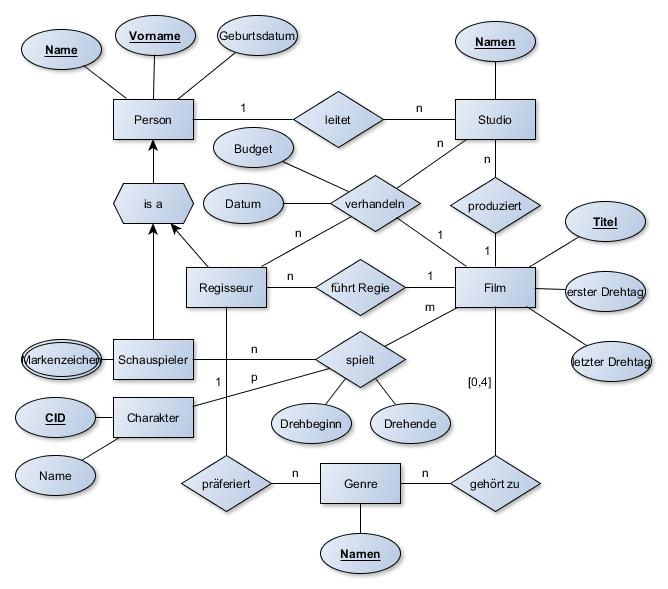
\includegraphics[width=180mm]{er_model.jpg}
                                \caption{ER-Model}
                                \label{overflow}
                            \end{figure}

                        \item 
                            Schauspieler präferiert ein bestimmtes Genre.\\
                            Schauspieler = Regisseur\\
                            Filme mit bestimmten Titel können nur von einem bestimmten Studio gemacht werden.\\
                            Filmreihen.\\
                            Regisseur Verhandlung mindestes Budget.\\
                \end{enumerate} 
        \item
            \begin{enumerate}
                \item  
                    \begin{itemize}
                        \item Ein Schüler hat eine eindeutige MatrikelNr und einen Namen.
                        \item Die Studiengänge besitzten einen eindeutigen Namen.
                        \item Ein Student ist in genau einem Studiengang immatrikuliert.
                        \item In einem Sutdiengang sind n Studenten immatrikuliert.
                    \end{itemize} 
                \item   
                    \begin{itemize}
                        \item Universität hat einen eindeutigen Namen.
                        \item Ein Hörsaal besitzt einen eindeutigen Namen und und eine Anzahl Plätze.
                        \item Eine Universität besitzt mindestens ein Hörsaal.
                        \item Ein Hörsaal gehört genau zu einer Universität und kann ohne diese nicht existieren.
                    \end{itemize}
                \item   
                    \begin{itemize}
                        \item Ein Auftrag besitzt eine eindeutige ANR und ein Datum.
                        \item Ein Ersatzteil besitzt ein Automodell und einen  Namen und einen Preis.
                        \item Die Kombination aus Name und Automodell machen es eindeutig.
                        \item Reparaturtypen sind eindeutig an ihrer Art erkennbar und besitzen Art und einen Festpreis.
                        \item Bei jeder Reparatur werden n Aufträge gestellt, N Ersatzteile verwendet und o Reparaturtypen genutzt.
                        \item Die Reparaturen besitzen eine Uhrzeit und ein Datum.
                    \end{itemize}
                \item   
                    \begin{itemize}
                        \item Beliebig viele Mannschaften spielen in Spielen in einen Fußballspiele gegen Beliebig \\
                        viele andere Mannschaft in Beliebig vielen Stadien an denen Beliebig viele Schiedsrichtern beteiligt sind.
                    \end{itemize}
             \end{enumerate}
        \item 
            \begin{enumerate}
                \item 
                    HausNr und Vorname ist keine gute Kombination da dies nicht eindeutig ist. Es existiert \\
                    zwei Einträge bei denen diese Kombination (Frida, 8) identisch sind. Ein Primärschlüssel \\
                    sollte eindeutig sein. Daher würde würde das Attribut Vorname in diesem Fall kein \\
                    Primärschlüssel sein, da Frida zweimal vorhanden ist. Ein Primärschlüssel sollte \\
                    wenigen Attributen bestehen. So wäre es am besten nur ein Attribut als Primärschlüssel\\
                     zu wählen, wie z.B. Vorname, aber dies verstößt gegen die Eindeutigkeit. Daher wäre es \\
                     sinnvoller Vorname in Kombination mit einem anderen Attribut zu wählen die eindeutig ist.\\
                    potenzielle Primärschlüssel: PLZ 2. Fach, Telefonnummer PLZ 
                \item
                    Die oben genannt Beispiele wären nicht toll. Da Studenten in der selben WG wohnen haben \\
                    sie folglich die gleiche Plz und Telefonnummer, etc. daher ist eine eindeutige Kombination \\
                    nötig. In diesem Kontext da die Wahrscheinlichkeit von gleichen Sachen zu hoch ist und\\
                     daher weitere Attribute zum Primärschlüssel hinzufügen was gegen minimal verstößt daher \\
                     wäre am sinnvollsten die Martikelnummer zu nutzen. \\
                    Ursache : WG dessen Ursache kein Geld  
            \end{enumerate}
    \end{enumerate}
\end{document}